\section*{Ensayo}

{
    \renewcommand{\labelitemi}{$\diamond$}
    \begin{itemize}
        \item \textbf{Comunicaci\'on dentro de la misma red - Etapa 1}
            \newline
            Aqu\'i se configuraron los dispositivos finales al switch. Se pidi\'o que la m\'ascara de subred
            fuese 255.255.255.252 y las direcciones IP para las PC's 192.168.0.2 y 192.168.0.5
            \begin{figure}[ht]
                \centering
                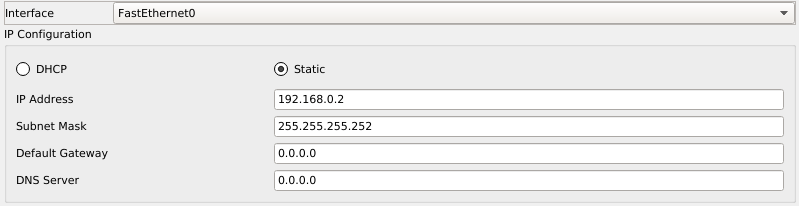
\includegraphics[width=12cm, height=5cm]{imagenes/captura1.png}
                \caption{Configuraci\'on para PC-1}
            
                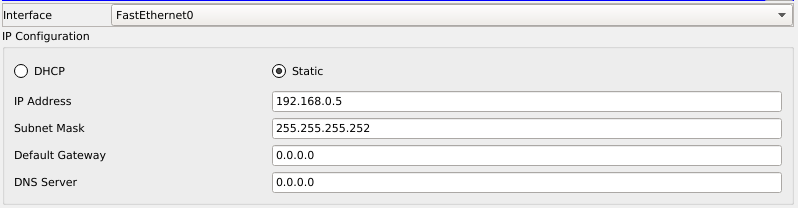
\includegraphics[width=12cm, height=5cm]{imagenes/captura2.png}
                \caption{Configuraci\'on para Laptop-1}
                
                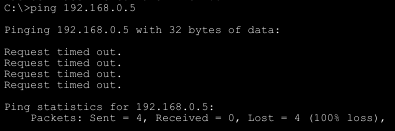
\includegraphics[width=12cm, height=5cm]{imagenes/captura3.png}
                \caption{Ping de PC-1 a Laptop-1}
            \end{figure}
            \newpage 
            \textbf{?`Por qu\'e se obtiene el resultado anterior?}
            \begin{itemize}
                \item[] El resultado anterior se debe a que la \textit{ip} 192.168.0.5 est\'a en otro segmento de red, 
                debido a la m\'ascara de red que se le asign\'o. Si se hubiese asignado la \textit{ip} 192.168.0.1 el ping 
                hubiese funcionado correctamente. Cuando el sufijo de la notaci\'on simplificada es /30 solo se puede
                hacer direccionamiento de 2 IP's (debido a que la primera \textit{ip} sirve para la direcci\'on de red y la ultima
                para direcci\'on de broadcast). \newline
                En cambio, s\'i se hubiese utilizado el sufijo /29 ya se tienen 6 direcciones disponibles y aqu\'i no es
                necesario cambiar la direcci\'on \textit{ip}.
            \end{itemize}
        
        \item \textbf{Comunicaci\'on dentro de la misma red - Etapa 2}
            \newline
            La m\'ascara de red que permitir\'ia la comunicaci\'on entre ambos dispositivos es 255.255.255.248. Esto hace que las 
            IP's 192.168.0.2 y 192.168.0.5 se encuentren en el mismo segmento de red, pues aqu\'i se pueden direccionar 6 IP's, el 
            sufijo de notaci\'on simplificada ser\'a /29.
            \begin{figure}[ht]
                \centering
                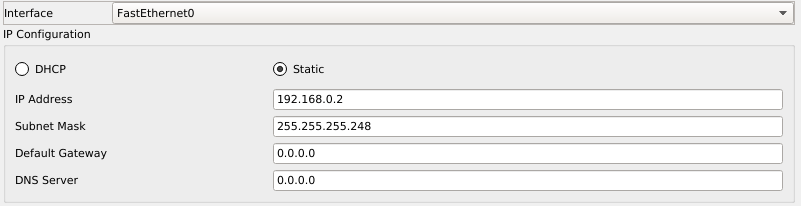
\includegraphics[width=12cm, height=5cm]{imagenes/captura4.png}
                \caption{Cambio de m\'ascara de red PC-1}

                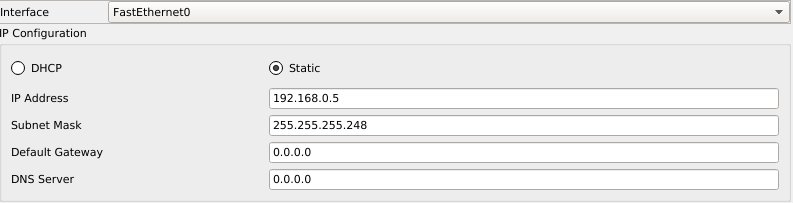
\includegraphics[width=12cm, height=5cm]{imagenes/captura5.png}
                \caption{Cambio de m\'ascara de red Laptop-1}
            \end{figure}
            \newpage
            \begin{figure}[ht]
                \centering
                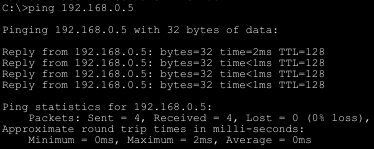
\includegraphics[width=12cm, height=5cm]{imagenes/captura6.png}
                \caption{ping de PC-1 a Laptop-1}
            \end{figure}
        \item \textbf{Comunicaci\'on entre redes - Etapa 3}
            \newline
            Configuraci\'on del router y las los dispositivos finales, asignaci\'on de las interfaces del router y los gateway de
            los dispositivos.
            
            \begin{figure}[ht]
                \centering
                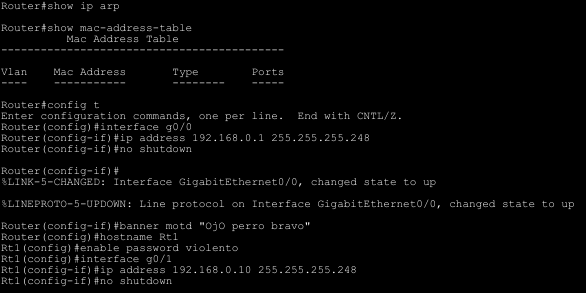
\includegraphics[width=12cm, height=5cm]{imagenes/captura7.png}
                \caption{Configuraci\'on de las interfaces del router}
                
                \begin{subfigure}[b]{0.4 \linewidth}
                    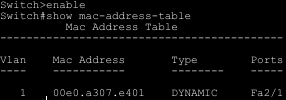
\includegraphics[width=6.2cm, height=3.5cm]{imagenes/captura8.png}
                    \caption{Switch-1}
                \end{subfigure}
                \begin{subfigure}[b]{0.4 \linewidth}
                    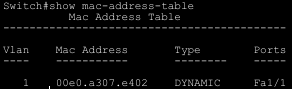
\includegraphics[width=6.2cm, height=3.5cm]{imagenes/captura9.png}
                    \caption{Switch-2}
                \end{subfigure}
                \caption{Informaci\'on de tabla MAC de los Switches}
            \end{figure}
            \newpage

            \begin{figure}[ht]
                \centering
                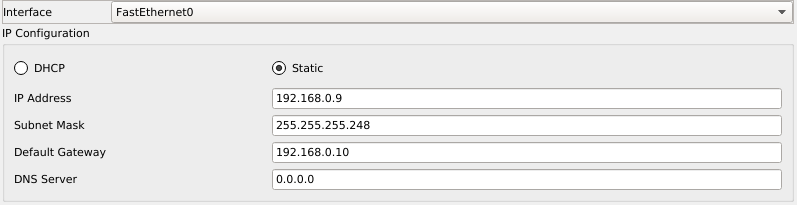
\includegraphics[width=12cm, height=5cm]{imagenes/captura10.png}
                \caption{Configuraci\'on de PC-2}
                
                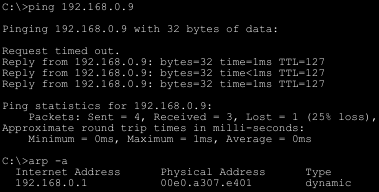
\includegraphics[width=12cm, height=5cm]{imagenes/captura12.png}
                \caption{Comunicaci\'on con PC-2 y Tabla ARP de PC-1}

                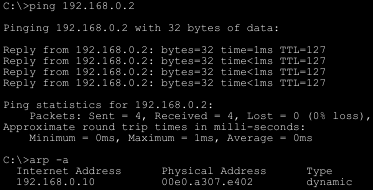
\includegraphics[width=12cm, height=5cm]{imagenes/captura13.png}
                \caption{Comunicaci\'on con PC-1 y Tabla ARP de PC-2}
            \end{figure}
            \newpage

            \begin{figure}[ht]
                \centering
                \begin{subfigure}[b]{0.4 \linewidth}
                    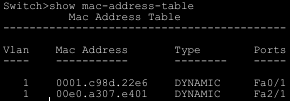
\includegraphics[width=6.2cm, height=3.5cm]{imagenes/captura14.png}
                    \caption{MAC de Switch-1}
                \end{subfigure}
                \begin{subfigure}[b]{0.4 \linewidth}
                    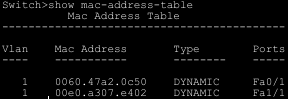
\includegraphics[width=6.2cm, height=3.5cm]{imagenes/captura15.png}
                    \caption{MAC de Switch-2}
                \end{subfigure}
                \begin{subfigure}[b]{0.4 \linewidth}
                    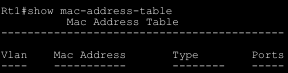
\includegraphics[width=6.2cm, height=3.5cm]{imagenes/captura16.png}
                    \caption{MAC de Router}
                \end{subfigure}
                \caption{Tablas MAC de switches y router}
            \end{figure}
    \end{itemize}

    \renewcommand{\labelitemi}{$\diamond$}
    \begin{itemize}
        \item \textbf{?`Cual es el prop\'osito de la m\'ascara de red?}
            \subitem La m\'ascara de red sirve para determinar el segmento de red disponible. Este segmento de red 
            tiene un rango disponible para conectar tantas IP's como se necesiten pero sin salir de ese rango. Si se 
            necesitan m\'as IP's se deben generar un rango que soporte m\'as direcciones. \newline
            Estas direcciones permiten que las m\'aquinas hagan referencia a su propia red sin conocer
            su n\'umero \textit{(pero tienen que conocer la m\'ascara de red para saber cu\'antos 0s incluir)}. La direcci\'on que
            consiste s\'olo en 1s, o 255.255.255.255 \textit{(la direcci\'on m\'as alta)}, se utiliza para indicar a todos los hosts
            en la red especificada. Permite la difusi\'on en la red local, por lo general una LAN. Las direcciones con
            un n\'umero de red apropiado y 1s en el campo de host permiten a las m\'aquinas enviar paquetes de
            difusi\'on a redes LAN distantes en cualquier parte de Internet \cite{Tanenbaum}. 

        \item \textbf{?`Porque las direcciones f\'isicas no tienen m\'ascara?}
            \subitem La direcci\'on MAC solo se necesita en el entorno f\'isico, es decir en la capa 2 del modelo OSI. El prop\'osito 
            de la m\'ascara de red es que una vez esten combinada con una direcci\'on IP se obtiene una direcci\'on \'unica en la red 
            donde se encuentra.\newline
            \newline
            Cuando al router que conecta varias redes le llega un paquete saca de \'el la dirección IP del host destino y realiza una 
            operaci\'on AND l\'ogica entre \'esta IP y las diferentes m\'ascaras de red de las redes que une, comprobando si el resultado 
            coincide con alguna de las direcciones propias de red \cite{Temas_para_la_educacion}. 
        \newpage

        \item \textbf{?`Que valores son v\'alidos para las m\'ascaras de red?}
            \subitem Los valores v\'alidos deben ser potencias de 2. Personalmente uso una f\'ormula para deducir los valores v\'alidos. 
            La f\'ormula es: 
            \begin{equation*}
                f(x) = 256 - 2^{x}  
            \end{equation*}
            Donde \textit{x} es el n\'umero de ceros que hay en la m\'ascara, de esta manera se puede saber que m\'ascara usar. Cabe mencionar 
            que la f\'ormula es una deducci\'on personal y solo funciona a nivel de octetos lo que significa que el valor que se le introduzca a 
            la funci\'on no puede ser mayor que 8.
        
        \item \textbf{?`Ser\'a posible comunicar dos espacios de red que tienen direcciones l\'ogicas diferentes?}
            \subitem S\'i es posible. Las direcciones l\'ogicas deber\'an \'ir asociadas a una m\'ascara de red, si la direcci\'on como un todo es 
            \'unica la red podr\'a comunicarse. En otras palabras si las direcciones IP's de un segmento de red no interfiere con las direcciones 
            de otro segmento la comunicaci\'on es posible.
    \end{itemize}
}